\documentclass[a4paper,12pt]{report}

\usepackage[russian]{config}

\usepackage{graphicx}
\usepackage{float}
\newcommand{\mytilde}{$\sim$}


% Description
\newcommand{\uniGroupName}{I2402}


\newcommand{\authorNameRu}{Балев Вадим}
\newcommand{\thesisTitleRu}{Исследование формата LaTeX и Git}
\newcommand{\thesisTypeRu}{практическая} 
\newcommand{\programulDeStudiiRu}{лиценциата} 
\newcommand{\identificatorulCursuluiRu}{информатика} 
\newcommand{\conducatorNameRu}{Курманский Антон}


\renewcommand{\year}{2025}
\newcommand{\github}{\url{https://github.com/BlackRoseGarotte/Practical_Work}}
\newcommand{\outputDate}{\today}

\begin{document}

%Titulnik
\titlePage

%Содержание
\clearpage
\tableofcontents

%Введение
\clearpage
\introChapter


\textbf{Актуальность использования LaTeX}

В современной документации, особенно при разработке программного обеспечения, инструменты LaTeX и Git обеспечивают высокую точность, контроль версий и удобство совместной работы.
LaTeX незаменим при создании документов с математическими формулами, таких как сложные уравнения, матрицы или интегралы, автоматической нумерацией разделов, таблиц и иллюстраций, а также сквозными ссылками на них и оглавлением. Он позволяет сосредоточиться на содержании, а не на оформлении, гарантируя соответствие издательским стандартам научных трудов.
Для работы был использован заготовленный преподавателем шаблон LaTex, для упощения работы студента, который не изучал ранее синтаксис этого языка(то есть меня).
Git, в свою очередь, помогает отслеживать изменения, работать в команде и управлять версиями проекта. Благодаря ветвлениям (branch) можно параллельно развивать разные части проекта — например, стабильную и экспериментальную версии. Операции merge и rebase позволяют безопасно объединять правки, сохраняя историю изменений прозрачной и управляемой.

Совместное использование LaTeX и Git особенно эффективно при подготовке сложных отчётов: это даёт возможность точно контролировать содержание документа и одновременно сохранять полную историю его разработки.


\textbf{Цель и задачи LaTeX}


Целью данной работы является изучение возможностей системы вёрстки  LaTex и освоение базовых приёмов работы с системой контроля версий Git, включая использование ветвлений (Git Branch).

Для достижения поставленной цели были сформулированы следующие \textbf{задачи}:


\textbf{Изучение Git и Git Branch LaTeX}

В рамках работы над проектом особое внимание было уделено изучению системы контроля версий Git, а также механизму ветвлений — \texttt{Git Branch}.

Git позволяет эффективно управлять изменениями в проекте, отслеживать историю версий, работать над различными частями проекта параллельно и безопасно сливать изменения. 

Механизм ветвлений (\texttt{branch}) является одной из ключевых возможностей Git. Он позволяет:

\begin{itemize}
    \item Создавать отдельные рабочие ветки для реализации новых функций или тестирования изменений;
    \item Разграничивать стабильную версию проекта и экспериментальные;
    \item Объединять изменения из разных веток при помощи слияния (\texttt{merge}) или ребейза (\texttt{rebase});
    \item Повышать надёжность и прозрачность процесса разработки.
\end{itemize}

Во время выполнения работы использовались следующие основные команды Git:

\begin{verbatim}
git init
git add .
git commit 
git branch 
git checkout 
git merge 
git rebase
git cherry-pick
git clone
git fetch

\end{verbatim}

Git стал одним из онсовных инструментом в процессе подготовки отчёта, обеспечивая как резервное копирование, так и удобное отслеживание прогресса.


\textbf{Практическое задание: интерактивное изучение ветвлений Git LaTeX}

В качестве практического задания была пройдена обучающая игра по Git-ветвлениям, доступная на сайте \url{https://learngitbranching.js.org/?locale=ru_RU}. 

Прохождение симулятора помогло закрепить знания о механике ветвлений в Git, научиться уверенно ориентироваться в древовидной структуре коммитов и применять различные стратегии объединения изменений. Благодаря пошаговому обучению, визуальной обратной связи и интерактивности, игра стала эффективным и наглядным способом освоения Git Branch.




%Глава 1
\chapter{LaTeX: система вёрстки документов}

\section{Введение в LaTeX}

LaTeX — это высококачественная система компьютерной вёрстки, ориентированная в первую очередь на создание научных и технических документов. Основное преимущество  LaTex заключается в чётком разделении содержимого и оформления, что позволяет автору сосредоточиться на содержании документа, а не на его внешнем виде.

\section{Основные возможности LaTeX}

LaTeX предоставляет следующие возможности:
\begin{itemize}
    \item Поддержка математической нотации любой сложности;
    \item Создание структурированных документов с главами, разделами, списками, таблицами и рисунками;
    \item Автоматическая генерация оглавления, списков таблиц и рисунков;
    \item Кросс-ссылки и библиография;
\end{itemize}

\section{Синтаксис LaTeX}

LaTeX использует разметку на основе текстовых команд, что делает его похожим на написание README-файлов в Markdown — структура документа описывается простым текстом, а финальный вид формируется автоматически. Однако, в отличие от Markdown, LaTeX обладает гораздо более мощными возможностями для типографски точного форматирования, особенно при работе с математикой, библиографией и сложной структурой документов.

\begin{verbatim}
Преамбула (до \begin{document})

\documentclass[опции]{класс}: Тип документа (report, article, book) и общие настройки (a4paper, 12pt).
Пример: \documentclass[a4paper,12pt]{report}
\usepackage[опции]{пакет}: Подключение функционала.
Примеры: \usepackage[russian]{babel}, \usepackage{graphicx}, \usepackage{amsmath}
\title{...}, \author{...}, \date{...}: Информация для титульного листа.
Тело документа (между \begin{document} и \end{document})

Структура:
\chapter{Глава} (для report/book)
\section{Раздел}
\subsection{Подраздел}
\tableofcontents: Оглавление.
Текст:
\textbf{жирный}, \textit{курсив}, \underline{подчеркнутый}, \texttt{код}.
\\: Перенос строки.

Списки:

Ненумерованный (itemize):

\begin{itemize}
    \item Пункт 1
    \item Пункт 2
\end{itemize}

Нумерованный (enumerate):

\begin{enumerate}
    \item Пункт 1
    \item Пункт 2
\end{enumerate}

\section{Заключение}
\end{verbatim}




\section{Практическое использование LaTeX в работе над отчётом}

В процессе подготовки данного отчёта я использовал LaTeX в рабочей среде  Linux на базе виртуальной среде Windows Subsystem for Linux (WSL), так как LaTex работает гораздо менее стабильнее Windows.

\subsection{Среда разработки}

Для написания и компиляции LaTeX-документа была настроена следующая среда:

\begin{itemize}
    \item \textbf{WSL} — технология от Microsoft, позволяющая запускать Linux-дистрибутивы непосредственно в Windows без использования виртуальной машины;
    \item \textbf{Ubuntu} — выбранный дистрибутив Linux, установленный в WSL;
    \item \textbf{TeX Live} — дистрибутив  LaTex, установленный в Ubuntu;
    \item \textbf{Visual Studio Code} — основной текстовый редактор, использовавшийся для редактирования исходников;
\end{itemize}

\subsection{Установка LaTeX}

В Ubuntu установка LaTeX производилась следующей командой:

\begin{verbatim}
sudo apt update
sudo apt install fonts-liberation xz-utils texlive-bibtex-extra biber texlive texlive-lang-cyrillic texlive-lang-european python3-pygments latexmk texlive-xetex # liberation font, font utils, latex, python
curl -L -O https://notabug.org/ArtikusHG/times-new-roman/raw/master/times.tar.xz
sudo tar -xf times.tar.xz -C /usr/share/fonts/
fc-cache -f -v
\end{verbatim}

\subsection{Преимущества такой среды}

Использование WSL и Ubuntu позволило использовать мощные инструменты Linux в привычной среде Windows.

\subsection{Заключение}

Такой подход позволил мне эффективно использовать возможности LaTeX в подготовке структурированного отчёта, комбинируя эффективность Linux-среды с удобством редактора VS Code.






%Глава 2
\chapter{Работа с GitBranch}

%2.1
\section{О платформе LearnGitBranching}

 LearnGitBranching — это бесплатная интерактивная веб-платформа, предназначенная для изучения системы контроля версий Git.

Основной особенностью платформы является визуализация веток и истории коммитов в реальном времени. Это позволяет пользователю наглядно видеть результат выполнения каждой команды Git и формировать интуитивное понимание структуры репозитория.

На сайте представлены обучающие уровни, в которых необходимо выполнить определённые задачи с использованием командной строки Git. Уроки охватывают как базовые операции (создание коммитов, веток, слияние), так и более продвинутые темы (rebase, cherry-pick, reset).

Команды Git
В песочнице можно использовать множество команд:

commit
branch
checkout
cherry-pick
reset
revert
rebase
merge
clone
push
pull


\section{Ход работы}

\subsection{Шаг 1}
Для прохождения этого уровня нужно было просто дважды ввести \textbf{git commit}, чтобы создать 2 узла.

\begin{figure}[H]
    \centering
    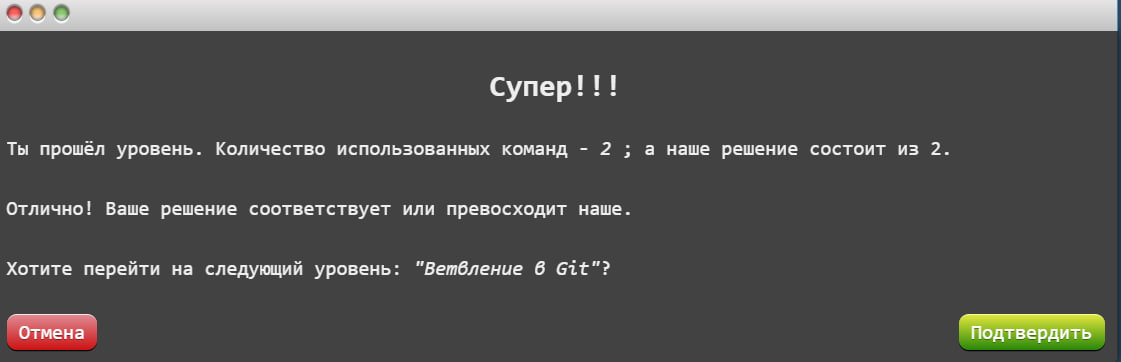
\includegraphics[width=0.75\textwidth]{images/step1.jpg} 
\end{figure}

\subsection{Шаг 2}

Ветки в Git, как и коммиты, невероятно легковесны. Это просто ссылки на определённый коммит — ничего более. Вот почему многие фанаты Git повторяют мантру

делай ветки сразу, делай ветки часто

Так как создание множества веток никак не отражается на памяти или жестком диске, удобнее и проще разбивать свою работу на много маленьких веток, чем хранить все изменения в одной огромной ветке.
Для прохождения этого уровня надо было создать новую ветку при помощи \textbf{git branch name} и перейди на неё при помощи \textbf{git checkout name}.

\begin{figure}[H]
    \centering
    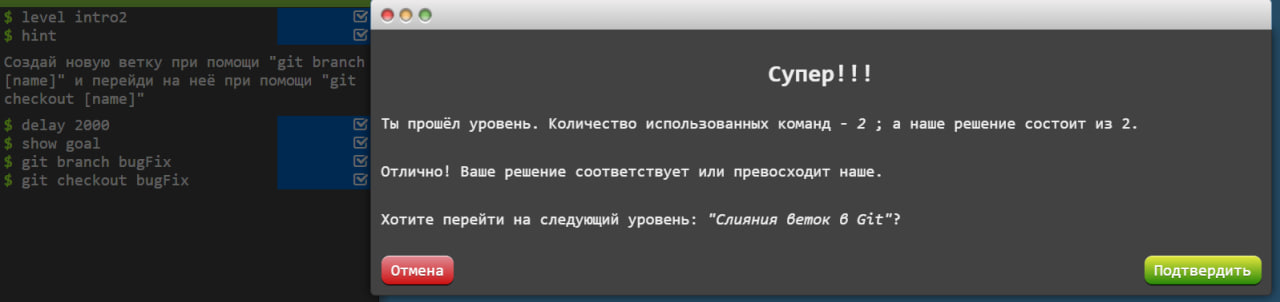
\includegraphics[width=0.75\textwidth]{images/step2.jpg} 
\end{figure}

В задаче требовалось создать ветку bugFix и перейти в нее.

\subsection{Шаг 3}

Ок! Мы уже знаем, как создавать ветки и коммитить наши изменения. Теперь надо понять, как объединять изменения из двух разных веток. Очень удобно создать ветку, сделать свою часть работы в ней и потом объединить изменения из своей ветки с общими.

Первый способ объединения изменений, который мы рассмотрим - это git merge - слияние или просто мердж. Слияния в Git создают особый вид коммита, который имеет сразу двух родителей. Коммит с двумя родителями обычно означает, что мы хотим объединить изменения из одного коммита с другим коммитом и всеми их родительскими коммитами.

\begin{figure}[H]
    \centering
    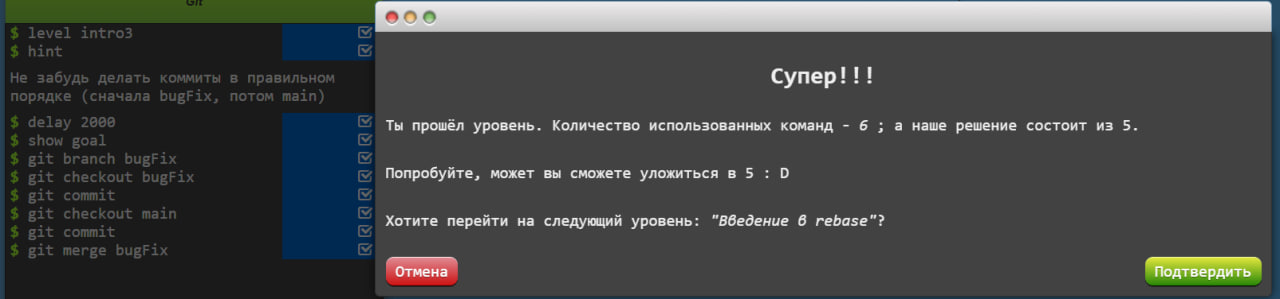
\includegraphics[width=0.75\textwidth]{images/step3.jpg} 
\end{figure}

Над этим уровнем надо было подумать, чтобы разобраться как работает слияние с помощью merge.

\subsection{Шаг 4}

Второй способ объединения изменений в ветках - это rebasing. При ребейзе Git по сути копирует набор коммитов и переносит их в другое место.

Несмотря на то, что это звучит достаточно непонятно, преимущество rebase в том, что c его помощью можно делать чистые и красивые линейные последовательности коммитов. История коммитов будет чище, если вы применяете rebase.

\begin{figure}[H]
    \centering
    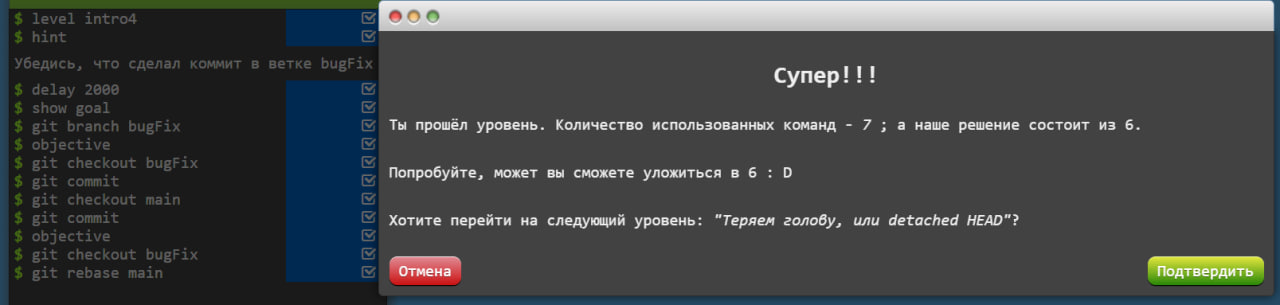
\includegraphics[width=0.75\textwidth]{images/step4.jpg} 
\end{figure}

Для меня этот метод оказался менее очевидным, так как во отличие от merge, визуально не сразу понятно как он работает. Merge был представлен буквально как слияние двух веток, что, по-моему, более наглядно.

\subsection{Шаг 5}

В первую очередь, поговорим о "HEAD". HEAD - это символическое имя текущего выбранного коммита — это, по сути, тот коммит, над которым мы в данный момент работаем.
HEAD всегда указывает на последний коммит из вашего локального дерева. Большинство команд Git, изменяющих рабочее дерево, начнут с изменения HEAD.

Обычно HEAD указывает на имя ветки например, bugFix. Когда вы делаете коммит, статус ветки bugFix меняется и это изменение видно через HEAD.

\begin{figure}[H]
    \centering
    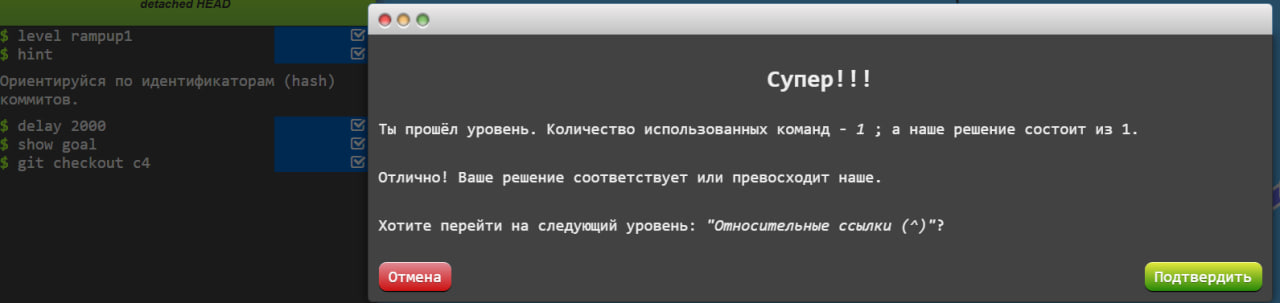
\includegraphics[width=0.75\textwidth]{images/step5.jpg} 
\end{figure}

Эта задача не вызвала проблем, был разобран указатель на коммиты. Он также является введением в hash, что так же не вызвало проблем.

\subsection{Шаг 6}

Передвигаться по дереву Git при помощи указания хешей коммитов немного неудобно. В реальной ситуации у вас вряд ли будет красивая визуализация дерева в терминале, так что придётся каждый раз использовать git log, чтобы найти хеш нужного коммита
Более того, хеши в реальном репозитории Git намного более длинные. Например, хеш для коммита, который приведён в предыдущем уровне - fed2da64c0efc5293610bdd892f82a58e8cbc5d8. Не очень просто для произношения
Хорошая новость в том, что Git достаточно умён в работе с хешами. Ему нужны лишь первые несколько символов для того, чтобы идентифицировать конкретный коммит. Так что можно написать просто fed2 вместо колбасы выше.

Как мы уже говорили, указание на коммит при помощи его хеша - не самый удобный способ, поэтому Git поддерживает относительные ссылки и они прекрасны!
С относительными ссылками можно начать с какого-либо удобного места например, с ветки bugFix или от HEAD и двигаться от него
Относительные ссылки - мощный инструмент, но мы покажем два простых способа использования:



%Не работает почему-то
%Перемещение на один коммит назад: коретка \texttt{\mytilde}
%Перемещение на несколько коммитов назад \texttt{~<num>}


\begin{figure}[H]
    \centering
    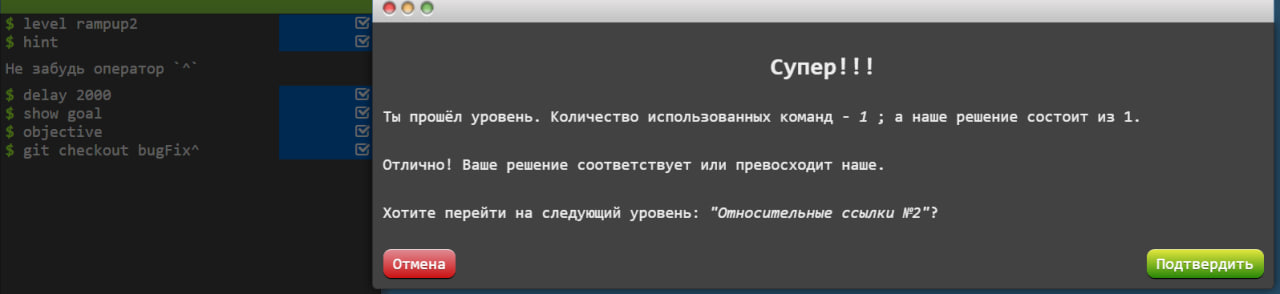
\includegraphics[width=0.75\textwidth]{images/step6.jpg} 
\end{figure}

Я использовал команды Git, чтобы изменить структуру веток и их положение. Я перемещал указатели веток на нужные коммиты, переключался между ветками и перестраивал историю коммитов, чтобы получить заданный результат.

\subsection{Шаг 7}

Предположим, нужно переместиться на много шагов назад по дереву. Было бы неудобно печатать тильду несколько раз или несколько десятков раз, так что Git поддерживает также оператор \mytilde.
К тильде опционально можно добавить количество родительских коммитов, через которые нужно пройти. Посмотрим, как это работает.

\begin{figure}[H]
    \centering
    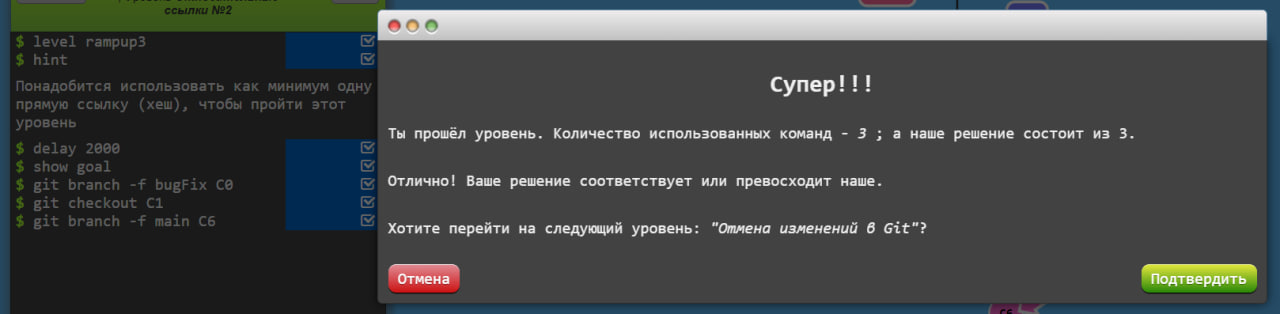
\includegraphics[width=0.75\textwidth]{images/step7.jpg} 
\end{figure}

Я выполнял команды Git, чтобы **изменить структуру и положение веток в моём репозитории**. Мои действия включали **перемещение указателей веток на нужные коммиты, а также создание новых коммитов** для достижения желаемой конфигурации истории.

\subsection{Шаг 8}

Есть много путей для отмены изменений в Git. Так же как и коммит, отмена изменений в Git возможна и на низком уровне (добавление в коммит отдельных файлов и наборов строк), и на высоком (как изменения реально отменяются). Сейчас сфокусируемся на высокоуровневой части.
Есть два основных способа отмены изменений в Git: первый - это git reset, а второй - git revert. Попробуем оба на следующем шаге.

\begin{figure}[H]
    \centering
    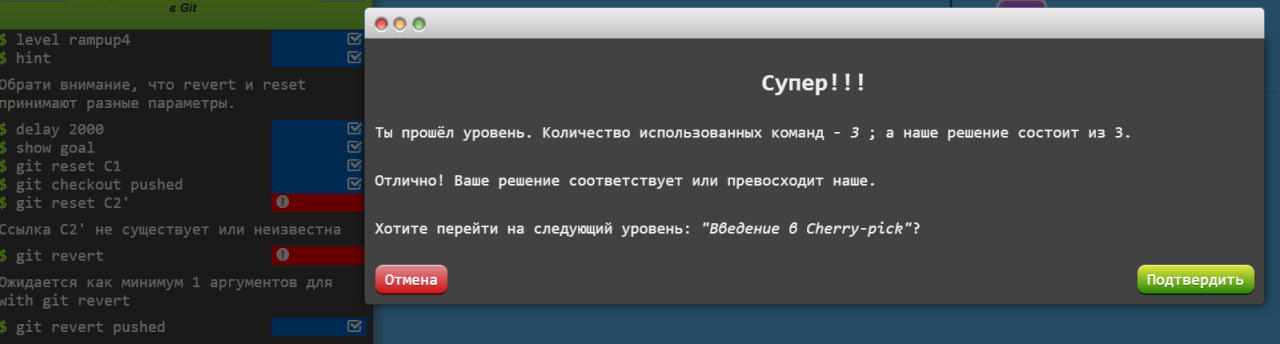
\includegraphics[width=0.75\textwidth]{images/step8.jpg} 
\end{figure}

Я использую команду git cherry-pick, чтобы выборочно применять изменения из указанных коммитов (c3, c4, c7) к моей текущей ветке. Это позволяет мне создавать новые коммиты с этими изменениями в текущей истории, не затрагивая исходные ветки или их структуру.

\subsection{Шаг 9}

Итак, мы уже освоили основы Git: коммиты, ветки, перемещение по дереву изменений. Уже этих знаний достаточно, чтобы овладеть 90 процентов мощи Git-репозиториев и покрыть нужды разработчиков.
А оставшиеся 10 процентов будут очень полезны при сложных workflow или если ты попал в сложную ситуацию. Теперь речь пойдёт о перемещении изменений — возможности, позволяющей разработчику сказать "Хочу, чтобы эти изменения были вот тут, а вот эти — вон там" и получить точные, правильные результаты, не теряя при этом гибкости разработки.

На первый взгляд запутанно, но на самом деле всё просто.

Первая из таких команд - это \textbf{git cherry-pick}. Она выглядит вот так:

\texttt{git cherry-pick <Commit1> <Commit2> <...>}

Это очень простой и прямолинейный способ сказать, что ты хочешь копировать несколько коммитов на место, где сейчас находишься (HEAD). Мы обожаем cherry-pick за то, что в нём очень мало магии и его очень просто понять и применять.

\begin{figure}[H]
    \centering
    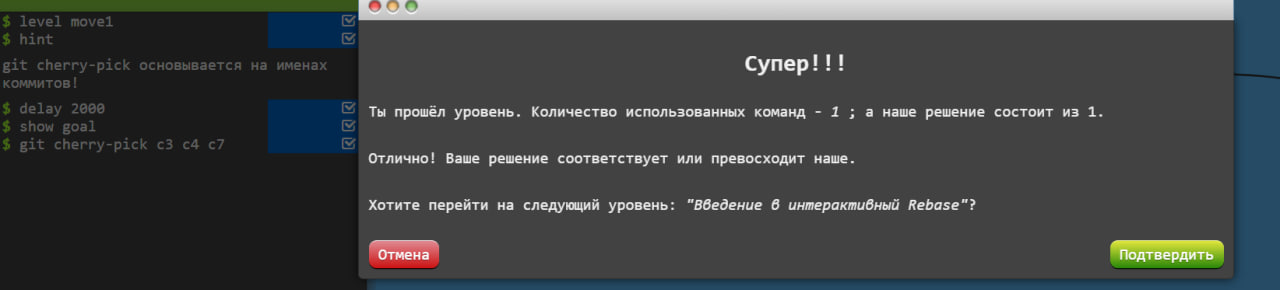
\includegraphics[width=0.75\textwidth]{images/step9.jpg} 
\end{figure}

\subsection{Шаг 10}

Git cherry-pick прекрасен, когда точно известно, какие коммиты нужны и известны их точные хеши
Но как быть в случае, когда точно не известно какие коммиты нужны? К счастью, Git позаботился о таких ситуациях! Можно использовать интерактивный rebase для этого - лучший способ отобрать набор коммитов для rebase.

Углубимся в детали.

Всё, что нужно для интерактивного rebase - это опция -i
Если добавить эту опцию, Git откроет интерфейс просмотра того, какие коммиты готовы к копированию на цель rebase (target). Также показываются хеши коммитов и комментарии к ним, так что можно легко понять что к чему.

\begin{figure}[H]
    \centering
    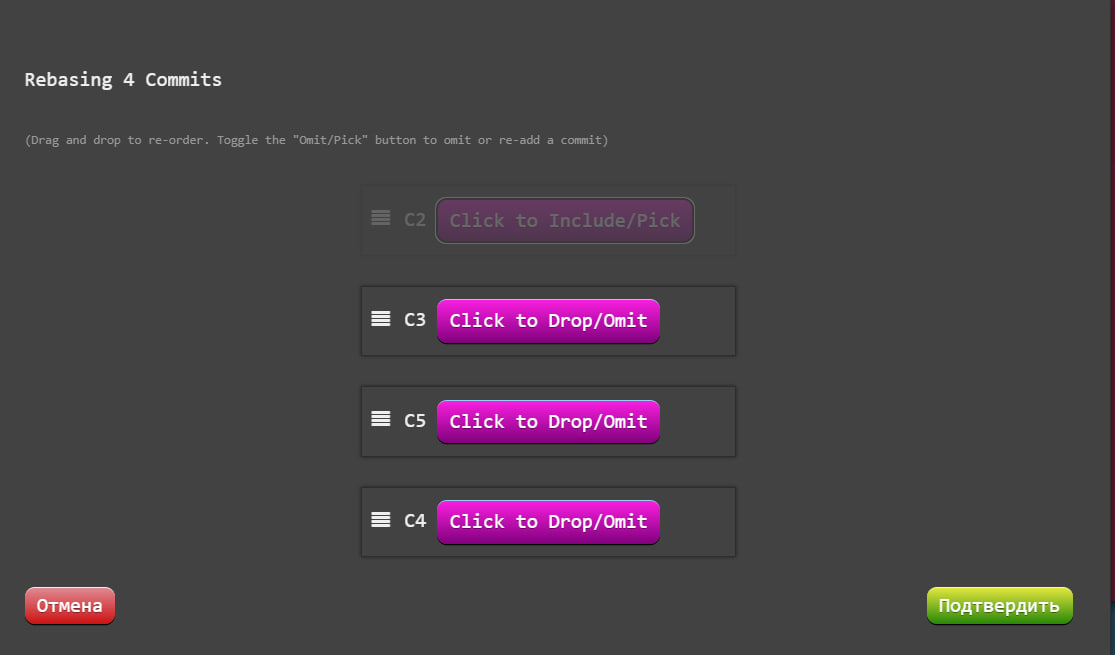
\includegraphics[width=0.75\textwidth]{images/step10_1.jpg} 
\end{figure}

\begin{figure}[H]
    \centering
    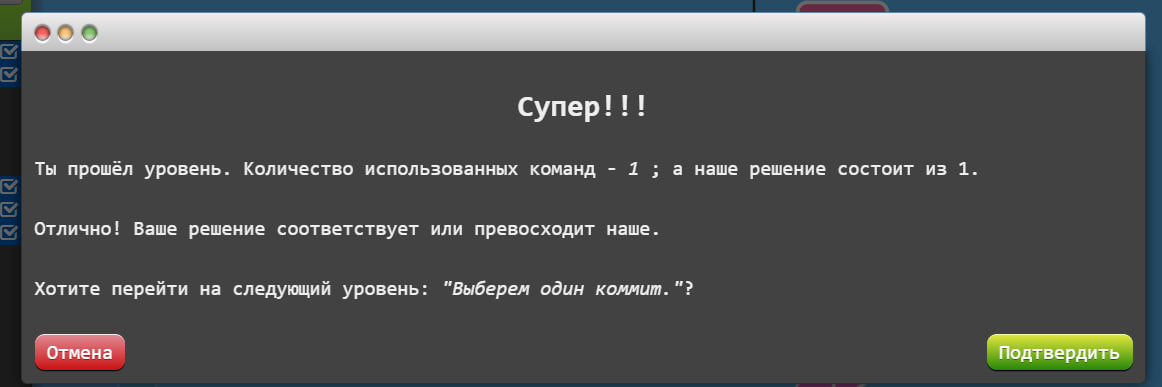
\includegraphics[width=0.75\textwidth]{images/step10_2.jpg} 
\end{figure}

Я использовал rebase -i, а после в открывшемся интерфейсе расположил все интуитивно.

\subsection{Шаг 11}

Вот ситуация, которая часто случается при разработке: мы пытаемся отследить ошибку, но она не очень очевидна. Для того, чтобы достичь успеха на этом поприще, мы используем несколько команд для отладки и вывода
Каждая отладочная команда вывода находится в своём коммите. В итоге мы нашли ошибку, исправили её и порадовались!
Но проблема в том, что мы хотим добавить в main только исправление ошибки из ветки bugFix. Если мы воспользуемся простым fast-forward, то в main попадут также отладочные команды. Должен быть другой способ...


\begin{figure}[H]
    \centering
    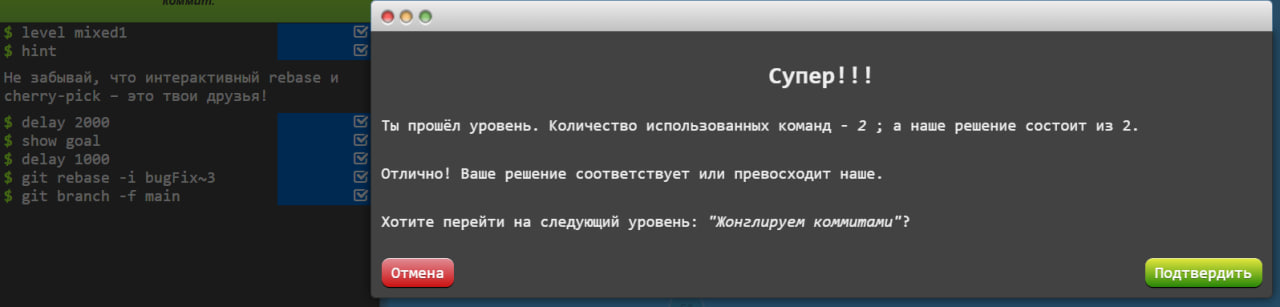
\includegraphics[width=0.75\textwidth]{images/step11.jpg} 
\end{figure}

Я использую команды git rebase -i и git branch -f, чтобы перестроить историю коммитов и переместить ветку main. Эти действия позволяют мне изменить структуру и положение веток в репозитории, достигая необходимой конфигурации истории.

\subsection{Шаг 12}

Вот ещё одна ситуация, которая часто случается. Есть некоторые изменения newImage и другие изменения caption, которые связаны так, что находятся друг поверх друга в репозитории.

Штука в том, что иногда нужно внести небольшие изменения в более ранний коммит. В таком случае надо немного поменять newImage, несмотря на то, что коммит уже в прошлом!

\begin{figure}[H]
    \centering
    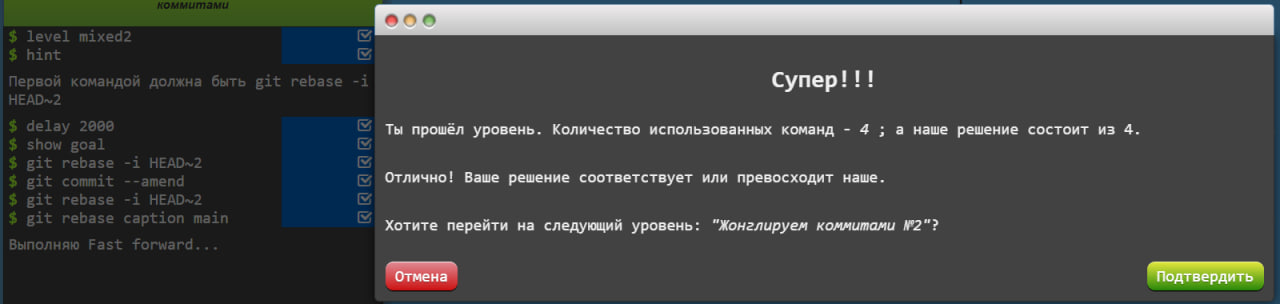
\includegraphics[width=0.75\textwidth]{images/step12.jpg} 
\end{figure}

Я выполняю последовательность команд Git, включая git checkout main, git cherry-pick C2, git commit --amend, и git cherry-pick C3. Моя цель — перестроить историю коммитов и переместить ветку main на новую, модифицированную цепочку, добиваясь определённой структуры в репозитории.

\subsection{Шаг 13}

В прошлом уровне мы использовали rebase -i, чтобы переставлять коммиты. Как только нужный нам коммит оказывался в конце, мы могли спокойно изменить его при помощи --amend и переставить обратно.

Единственная проблема тут - это множество перестановок, которые могут спровоцировать конфликты. Посмотрим, как с этой же задачей справится cherry-pick.

\begin{figure}[H]
    \centering
    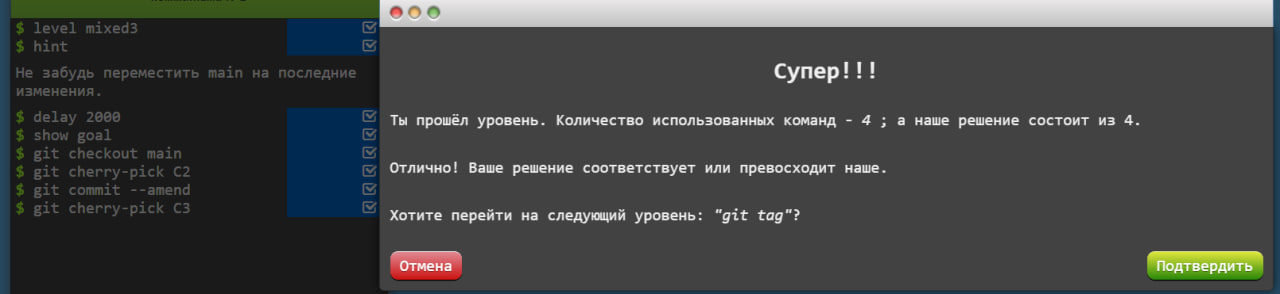
\includegraphics[width=0.75\textwidth]{images/step13.jpg} 
\end{figure}

 Я выполняю последовательность команд Git, включая git checkout main, git cherry-pick C2, git commit --amend, и git cherry-pick C3. Моя цель — перестроить историю коммитов и переместить ветку main на новую, модифицированную цепочку, добиваясь определённой структуры в репозитории.
\subsection{Шаг 14}

В прошлых уроках мы усвоили, что ветки просто двигать туда-сюда и они часто ссылаются на разные коммиты как на изменения данных в ветке. Ветки просто изменить, они часто временны и постоянно меняют своё состояние.

В таком случае, где взять постоянную ссылку на момент в истории изменений? Для таких вещей, как релиз и большие слияния, нужно нечто более постоянное, чем ветка.

Такое средство имеется. Git предоставляет нам теги, чья основная задача – ссылаться постоянно на конкретный коммит.
Важно, что после создания они никогда не сменят своего положения, так что можно с лёгкостью сделать checkout конкретного момента в истории изменений

\begin{figure}[H]
    \centering
    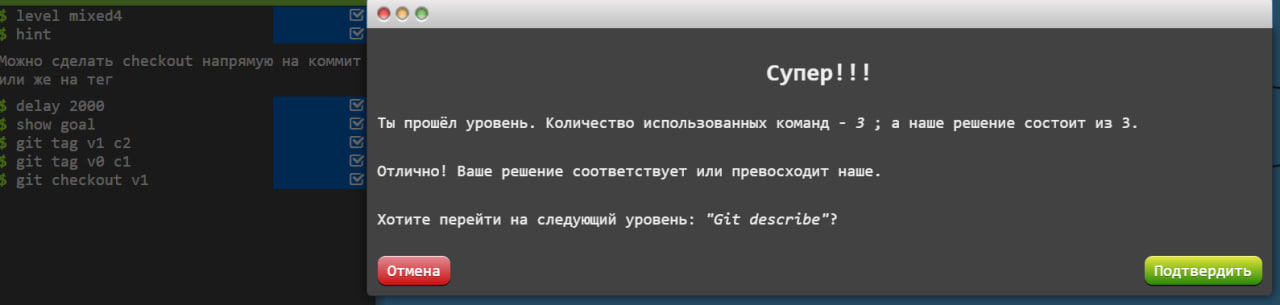
\includegraphics[width=0.75\textwidth]{images/step14.jpg} 
\end{figure}


Я создаю две именованные метки, v1 и v0, которые указывают на коммиты c2 и c1 соответственно. Затем я переключаюсь на метку v1, чтобы работать из этого конкретного состояния истории.
\subsection{Шаг 15}

Теги являются прекрасными ориентирами в истории изменений, поэтому в git есть команда, которая показывает, как далеко текущее состояние от ближайшего тега. И эта команда называется git describe

Git describe помогает сориентироваться после отката на много коммитов по истории изменений. Такое может случиться, когда вы сделали \texttt{git bisect}

Git describe выглядит примерно так:


\texttt{git describe ref}

Где ref — это что-либо, что указывает на конкретный коммит. Если не указать ref, то git будет считать, что указано текущее положение HEAD.

\begin{figure}[H]
    \centering
    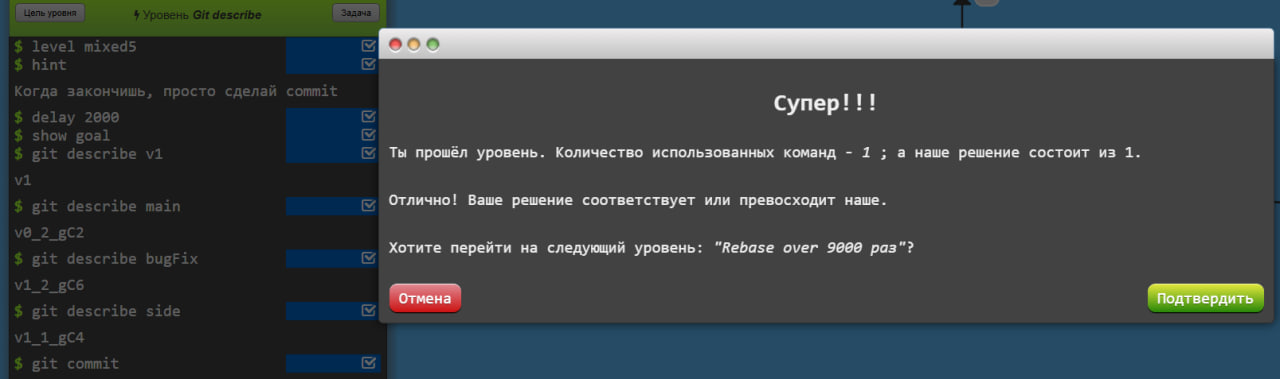
\includegraphics[width=0.75\textwidth]{images/step15.jpg} 
\end{figure}


Я использовал команду git describe для получения краткого, человекочитаемого названия ближайшего тега или коммита для различных веток (v1, main, bugFix, side). В конце я зафиксировал текущие изменения с помощью git commit, чтобы завершить уровень.

\subsection{Шаг 16}

У нас тут куча веток! Было бы круто перенести все изменения из них в мастер.
Но начальство усложняет нашу задачу тем, что желает видеть все коммиты по порядку. Так что коммит С7' должен идти после коммита С6' и так далее.

Если что-то пойдёт не так - можно использовать reset, чтобы начать всё с чистого листа. 

\begin{figure}[H]
    \centering
    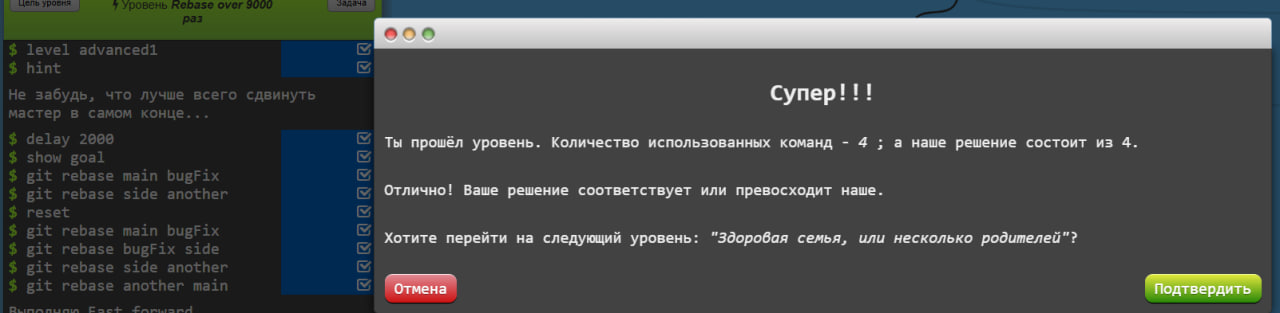
\includegraphics[width=0.75\textwidth]{images/step16.jpg} 
\end{figure}


Я выполняю несколько операций git rebase для последовательного перемещения веток bugFix, side, another относительно друг друга и main. Моя цель — перестроить сложную историю коммитов, чтобы main оказалась в нужном месте, используя эти перебазирования как основной инструмент.

\subsection{Шаг 17}

Так же как \mytilde, каретка принимает номер после себя.

Но в отличие от количества коммитов, на которые нужно откатиться назад, как делает \mytilde. Номер после каретки определяет, на какого из родителей мерджа надо перейти. Учитывая, что мерджевый коммит имеет двух родителей, просто указать каретку нельзя.
Git по умолчанию перейдёт на "первого" родителя коммита, но указание номера после каретки изменяет это поведение.

\begin{figure}[H]
    \centering
    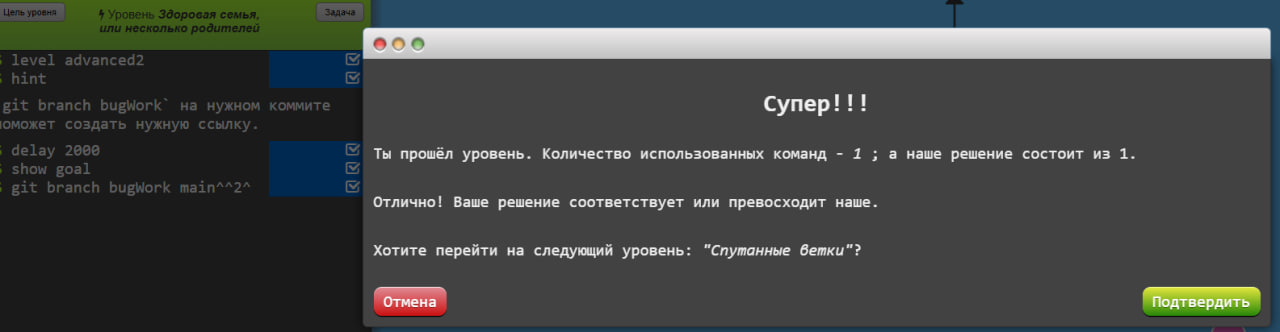
\includegraphics[width=0.75\textwidth]{images/step17.jpg} 
\end{figure}

Я вижу, что использую команду git branch bugWork main\mytilde\mytilde2\mytilde. Я создаю новую ветку под названием bugWork и размещаю её указатель на конкретном коммите, который находится в истории ветки main, отсчитывая несколько шагов назад.

\subsection{Шаг 18}

У нас тут по несколько коммитов в ветках one, two и three. Не важно почему, но нам надо видоизменить эти три ветки при помощи более поздних коммитов из ветки main.

Ветка one нуждается в изменении порядка и удалении C5. two требует полного перемешивания, а three хочет получить только один коммит

\begin{figure}[H]
    \centering
    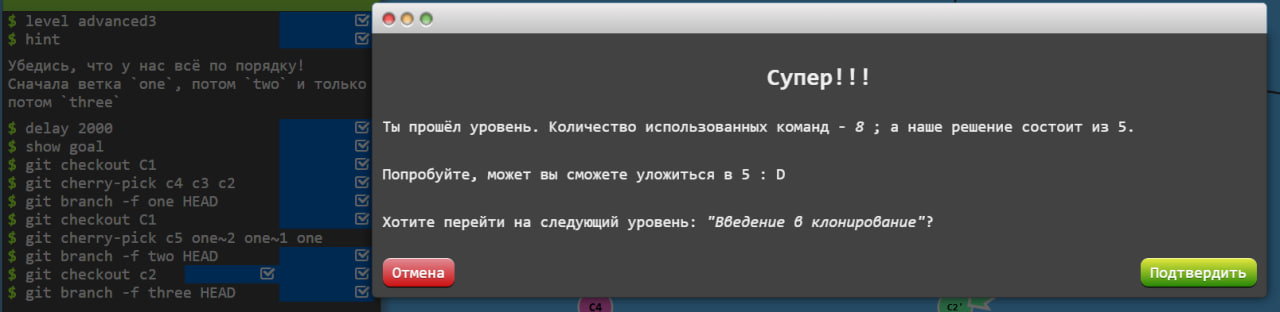
\includegraphics[width=0.75\textwidth]{images/step18.jpg} 
\end{figure}

Я выполнил серию команд Git, включая git checkout, git cherry-pick, и git branch -f. Моя цель — перестроить сложную структуру веток, создавая новые коммиты и перемещая указатели, чтобы добиться определённого расположения веток one, two, и three относительно коммитов C1, C2, C3, C4, C5.

\subsection{Шаг 19}

До настоящего момента мы были сфокусированы на изучении основ работы с локальным репозиторием ветвление, слияние, перемещение и т.д. Однако теперь, когда мы хотим научиться работать с удалёнными репозиториями, нам нужны новые команды для настройки рабочей среды для этих упражнений. Такой командой нам послужит git clone

Технически, \texttt{git clone} в реальной жизни - это команда, которая создаст локальную копию удалённого репозитория например, с GitHub. На наших занятиях в Learn Git Branching мы используем эту команду немного иначе - git clone создаёт удалённый репозиторий на основе вашего локального репозитория. На самом деле, это является полной противоположностью реальной команды, однако такой подход поможет нам наладить связь между склонированным и удалённым репозиторием. Давайте просто запустим эту команду.

\begin{figure}[H]
    \centering
    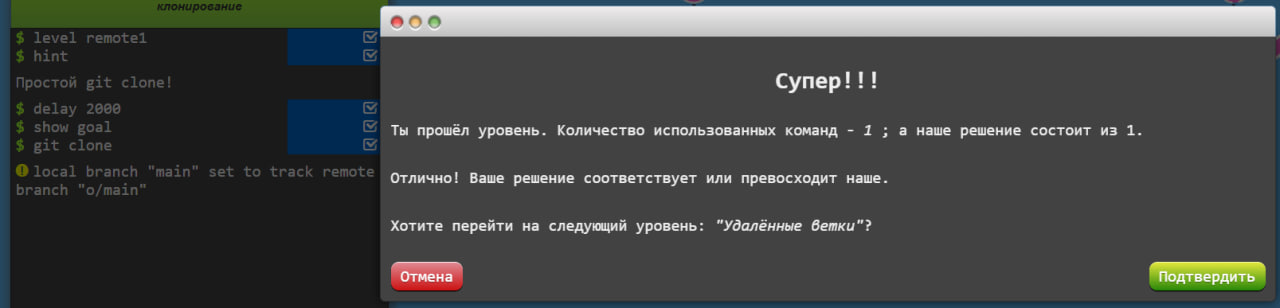
\includegraphics[width=0.75\textwidth]{images/step19.jpg} 
\end{figure}


Я выполнил команду git clone. Это действие создало локальную копию удалённого репозитория, автоматически настроив мою локальную ветку main на отслеживание удалённой ветки o/main.

\subsection{Шаг 20}

Теперь, когда мы уже увидели git clone в действии, давайте углубимся в детали и посмотрим что же на самом деле изменилось.

Во-первых, мы могли заметить, что у нас в локальном репозитории появилась новая ветка с именем o/main. Такой тип ветки называется удалённой веткой. Поскольку удалённые ветки играют важную и уникальную роль, они обладают рядом специальных свойств.
Удалённые ветки отражают состояние удалённых репозиториев с того момента, как вы обращались к этим удалённым репозиториям в последний раз. Они позволяют нам отслеживать и видеть разницу между нашими локальными наработками и тем, что было сделано другими участниками - важный шаг, который необходимо делать, прежде чем делиться своими наработками с другими.

Важным свойством удалённых веток является тот факт, что когда вы извлекаете их, вы отделяете detaching HEAD. Git делает это потому, что вы не можете работать непосредственно в этих ветках; сперва вам необходимо сделать наработки где-либо, а уж затем делиться ими с удалёнными репозиториями после чего наши удалённые ветки будут обновлены.

Что такое o/ в названии ветки?

Первый символ o/ в названии ветки служит для обозначения именно удалённых веток. Да. Удалённые ветки также имеют обязательное правило именования - они отображаются в формате:
Следовательно, если вы взглянете на имя ветки o/main, то здесь main - это имя ветки, а o - это имя удалённого репозитория.
Большинство разработчиков именуют свои главные удалённые репозитории не как o, а как origin. Также общепринятым является именование удалённого репозитория как origin, когда вы клонируете репозиторий командой git clone.

\begin{figure}[H]
    \centering
    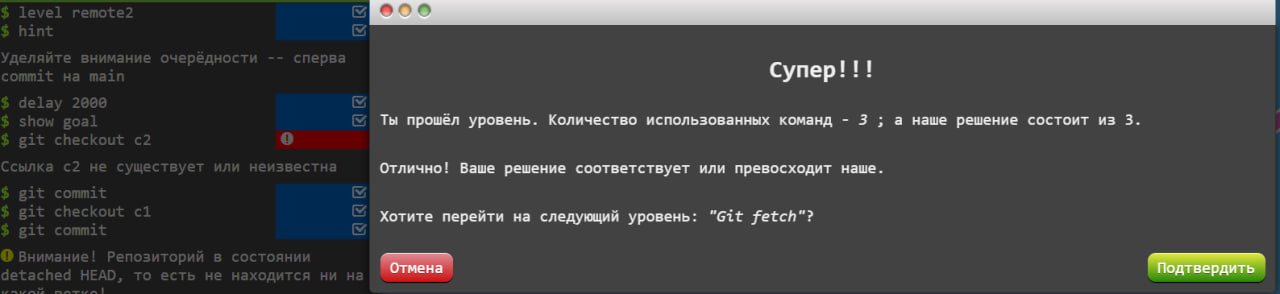
\includegraphics[width=0.75\textwidth]{images/step20.jpg} 
\end{figure}


Я использую команды git checkout и git commit, чтобы переключаться между коммитами и создавать новые. Однако, на скриншоте видно, что я столкнулся с ошибками, так как коммит c2 не был найден, и мне потребовался аргумент для git revert.

\subsection{Шаг 21}

Работа с удалёнными git репозиториями сводится к передаче данных в и из других репозиториев. До тех пор, пока мы можем отправлять коммиты туда-обратно, мы можем делиться любыми изменениями, которые отслеживает git следовательно, делиться новыми файлами, свежими идеями, любовными письмами и т.д..

В этом уроке вы научитесь тому, как извлекать данные из удалённого репозитория - и для этого у нас есть соответствующая команда \texttt{git fetch}.

\texttt{git fetch} выполняет две и только две основные операции. А именно:

связывается с указанным удалённым репозиторием и забирает все те данные проекта, которых у вас ещё нет, при этом...
у вас должны появиться ссылки на все ветки из этого удалённого репозитория (например, o/main)
Фактически, \texttt{git fetch} синхронизирует локальное представление удалённых репозиториев с тем, что является актуальным на текущий момент времени.

\begin{figure}[H]
    \centering
    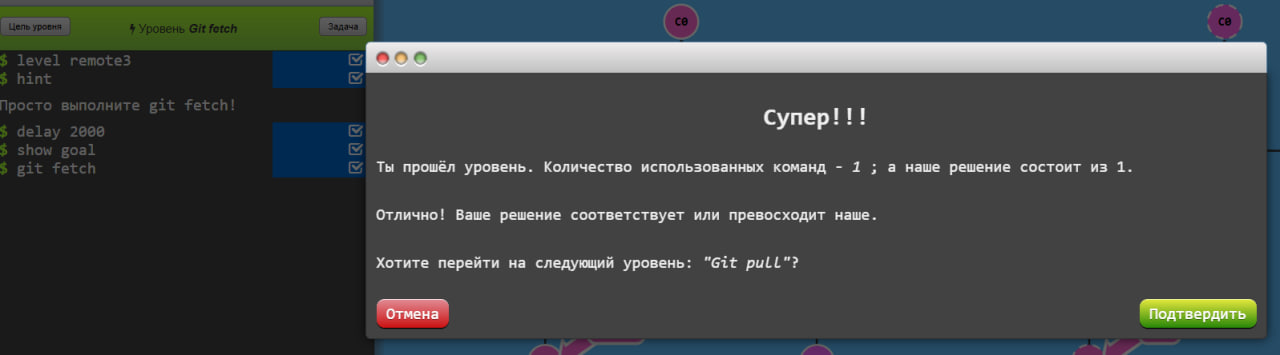
\includegraphics[width=0.75\textwidth]{images/step21.jpg} 
\end{figure}


Я выполняю команду git fetch. Моя цель — загрузить изменения с удалённого репозитория в мой локальный репозиторий, не объединяя их сразу с моими ветками.

\subsection{Шаг 22}

Теперь, когда мы познакомились с тем, как извлекать данные из удалённого репозитория с помощью git fetch, давайте обновим нашу работу, чтобы отобразить все эти изменения!

Существует множество вариантов решений - как только у вас имеется локальный коммит, вы можете соединить его с другой веткой. Это значит, вы можете выполнить одну из команд:

\texttt{git cherry-pick o/main}

\texttt{git rebase o/main}

\texttt{git merge o/main}

и т.д.

Процедура скачивания (fetching) изменений с удалённой ветки и объединения (merging) настолько частая и распространённая, что git предоставляет вместо двух команд - одну! Эта команда - \texttt{git pull}.

\begin{figure}[H]
    \centering
    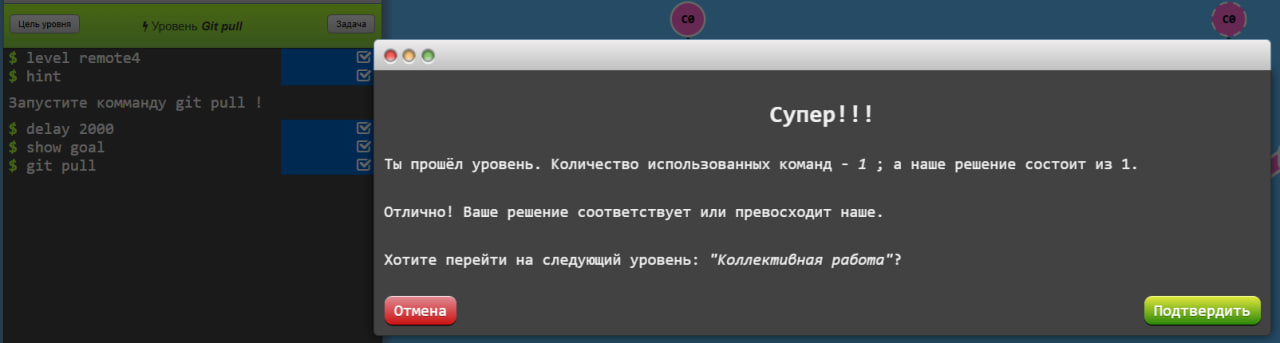
\includegraphics[width=0.75\textwidth]{images/step22.jpg} 
\end{figure}

Я использую команду git pull. Моя цель — загрузить изменения с удалённого репозитория и автоматически объединить их с моей текущей локальной веткой.

\subsection{Шаг 23}


\begin{figure}[H]
    \centering
    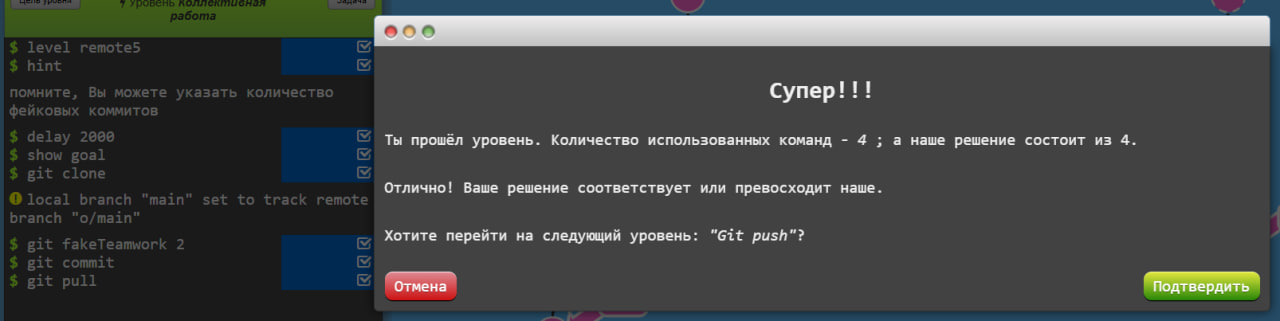
\includegraphics[width=0.75\textwidth]{images/step23.jpg} 
\end{figure}


Я выполнил команду git clone для создания локальной копии удалённого репозитория. После этого я использовал git fakeTeamwork 2 для симуляции совместной работы, добавил коммит с помощью git commit, а затем выполнил git pull, чтобы загрузить и объединить изменения из удалённого репозитория.

\subsection{Шаг 24}

Хорошо, мы скачали изменения с удалённого репозитория и включили их в наши локальные наработки. Всё это замечательно, но как нам поделиться своими наработками и изменениями с другими участниками проекта?
Способ, которым мы воспользуемся, является противоположным тому способу, которым мы пользовались ранее для скачивания наработок \texttt{git pull}. Этот способ - использование команды \texttt{git push}!

Команда \texttt{git push} отвечает за загрузку ваших изменений в указанный удалённый репозиторий, а также включение ваших коммитов в состав удалённого репозитория. По окончании работы команды git push все ваши друзья смогут скачать себе все сделанные вами наработки.
Мы можем рассматривать команду \texttt{git push} как "публикацию" своей работы. Эта команда скрывает в себе множество тонкостей и нюансов, с которыми мы познакомимся в ближайшее время, а пока что давайте начнём с малого...

\begin{figure}[H]
    \centering
    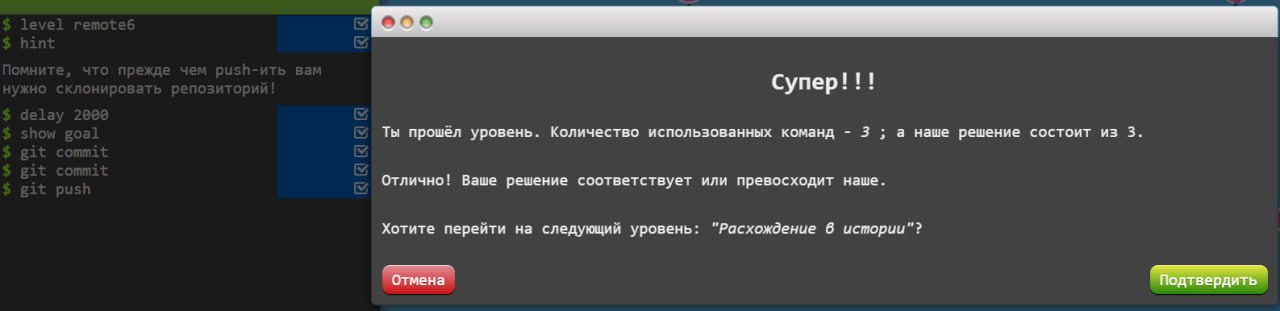
\includegraphics[width=0.75\textwidth]{images/step24.jpg} 
\end{figure}


Я создал два новых коммита, а затем отправил их изменения в удалённый репозиторий с помощью git push. Это действие обновило удалённую ветку до текущего состояния моей локальной ветки.

\subsection{Шаг 25}

Представим себе, что мы склонировали репозиторий в понедельник и начали разрабатывать какую-то новую и уникальную часть приложения (на сленге разработчиков - фича). В пятницу вечером мы наконец-то готовы опубликовать вашу фичу. Но, о нет! Наш коллега в течение недели написал кучу кода, который делает все наши наработки устарелыми. Этот код был также закоммичен и опубликован на общедоступном удалённом репозитории, поэтому теперь наш код базируется на устаревшей версии проекта и более не уместен.

В этом случае использование команды \texttt{git push} является сомнительным. Как поведёт себя команда \texttt{git push}, если вы её выполните? Может быть, она изменит удалённый репозиторий и вернёт всё к тому состоянию, которое было в понедельник? А может, команда попробует добавить наш код, не удаляя при этом новый? Или же она проигнорирует наши изменения, так как они уже устарели?

По причине того, что в данной ситуации (когда история расходится) слишком много двусмысленностей и неопределённостей, git не даст вам закачать (push) ваши изменения. Он будет принуждать вас включить в состав своей работы все те последние наработки и изменения, которые находятся на удалённом репозитории.

\begin{figure}[H]
    \centering
    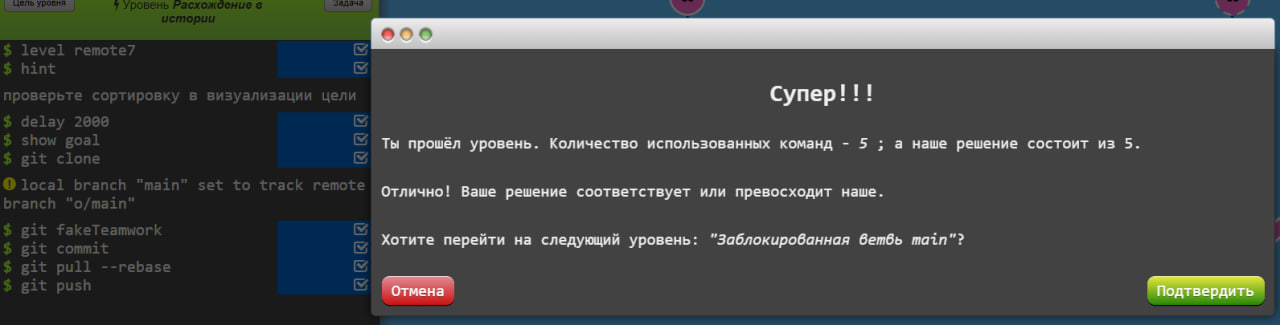
\includegraphics[width=0.75\textwidth]{images/step25.jpg} 
\end{figure}


Я выполнил серию команд Git, включая git clone, git fakeTeamwork, git commit, git pull --rebase и git push. Это позволило мне начать работу с удалённым репозиторием, симулировать изменения от коллег, а затем загрузить и отправить мои изменения, разрешая расхождения в истории с помощью перебазирования.

\subsection{Шаг 26}

\begin{figure}[H]
    \centering
    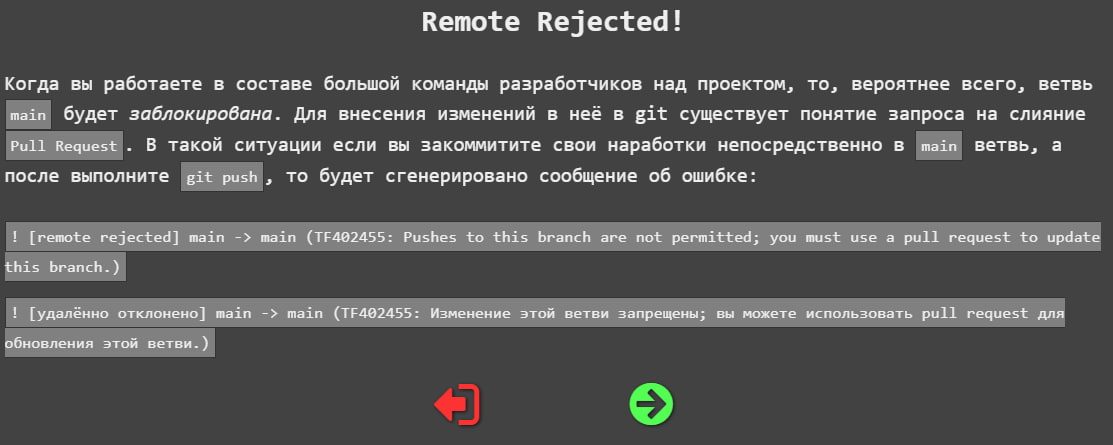
\includegraphics[width=0.75\textwidth]{images/remote_rejected.jpg} 
\end{figure}

Удалённый репозиторий отклонил загруженные коммиты непосредственно в main ветку потому, что на main настроена политика, которая требует использование Pull request вместо обычного git push.

Эта политика подразумевает процесс создания новой ветви разработки, внесение в неё всех необходимых коммитов, загрузка изменений в удалённый репозиторий и открытие нового Pull request. Однако вы забыли про это и закоммитили наработки непосредственно в main ветвь. Теперь вы застряли и не можете запушить свои изменения :(

\begin{figure}[H]
    \centering
    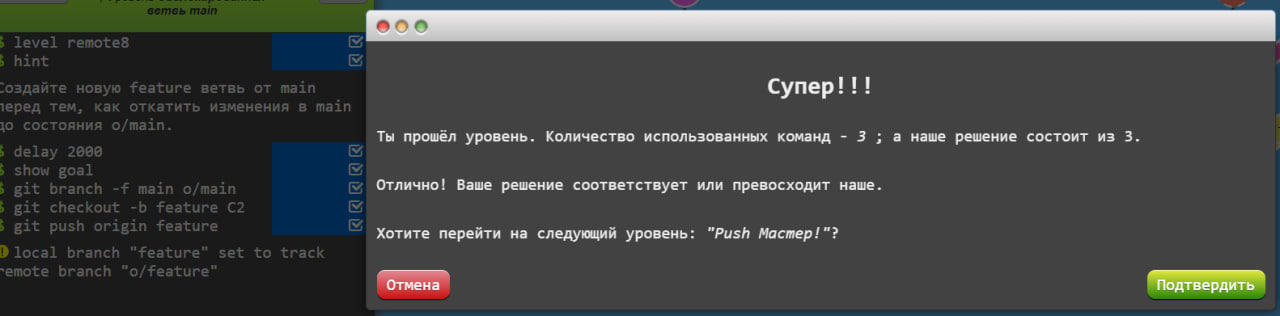
\includegraphics[width=0.75\textwidth]{images/step26.jpg} 
\end{figure}

Я создаю новую ветку feature от коммита C2, а затем откатываю ветку main до состояния, соответствующего удалённой ветке o/main. После этого я отправляю новую ветку feature в удалённый репозиторий.

\unnumberedChapter{Заключительные выводы}

В ходе проделанной работы были изучены LaTex и работа с Git. Использование LaTex позволяет автоматизировать процесс оформления отчета с помощью специального синтаксиса. LaTex позволяет использовать созданные программы или функции для оформления работы.
LaTex сложен для освоения с нуля, особенно при малом опыта работы с подобным инструментом. Он является более гибким аналогом прочих форматов (например markdown), позволяет настроить материал под себя.

Git, в свою очередь, является удобным инструментом для командного пронраммирования, так как он позволяет редактировать код локально, а после выгружать изменения на облако. Git предлагает широкий функционал, включая отслеживание изменений, слияние веток, возврат к предыдущим версиям и разрешение конфликтов.
Это делает его незаменимым для распределенной разработки, позволяя нескольким разработчикам одновременно работать над одним проектом, минимизируя риск потери данных и обеспечивая целостность кодовой базы. 

\textbf{Доступ к исходному коду:}

\github

\end{document}
% vim: fdm=syntax